\documentclass[12pt,twocolumn,letterpaper]{article}
%% Welcome to Overleaf!
%% If this is your first time using LaTeX, it might be worth going through this brief presentation:
%% https://www.overleaf.com/latex/learn/free-online-introduction-to-latex-part-1

%% Researchers have been using LaTeX for decades to typeset their papers, producing beautiful, crisp documents in the process. By learning LaTeX, you are effectively following in their footsteps, and learning a highly valuable skill!

%% The \usepackage commands below can be thought of as analogous to importing libraries into Python, for instance. We've pre-formatted this for you, so you can skip right ahead to the title below.

%% Language and font encodings
\usepackage[spanish,english]{babel}
\usepackage[utf8x]{inputenc}
\usepackage[T1]{fontenc}

%% Sets page size and margins
\usepackage[a4paper,top=3cm,bottom=2cm,left=2.5cm,right=2.5cm,marginparwidth=1.75cm]{geometry}

%% Useful packages
\usepackage{amsmath}
\usepackage{graphicx}
\usepackage[colorinlistoftodos]{todonotes}
\usepackage[colorlinks=true, allcolors=blue]{hyperref}
\usepackage{float}

%% Title
\title{
		%\vspace{-1in} 	
		\usefont{OT1}{bch}{b}{n}
		\normalfont \normalsize 
		\large \textbf{Checking Arc-Consistency of randomly generated graphs using four Arc-Consistency algorithms (AC-1, AC-2, AC-3, AC-4) } \\
}

\usepackage{authblk}
\author[0]{Mirajul Mohin, Roll: FH-028 
            
		}


\begin{document}
\maketitle

\selectlanguage{english}
\section*{Problem Description}
I have to select randomly generated graphs with random edges and select constraints for each edge from a constraint list, then run the Arc-Consistency algorithms (AC-1,AC-2, AC-3, AC-4) for increasing number of nodes and then measure the performances of each algorithm and plot a graph showing the comparison of four Arc-Consistency algorithms.

\section*{Experiment Setup}
All the AC algorithms are run in graphs that are randomly generated with the following properties:\\
- Number of nodes/variables are in range from 10 to 300 and increased by 10.\\
- Domain of each variable are in size 5 to 35 and each domain can have integers value ranging from 1 to 100.\\
- Constraints that at are used are as follows:\\\\ 1. X > Y\\
2. X < Y\\
3. X != Y \\
4. X = Y\textsuperscript{2} \\ \\
- If each value of domain of node\textsubscript{1}<15 and each value of domain of node\textsubscript{2}>15 then node\textsubscript{1} = node\textsubscript{2}\textsuperscript{2} is used. \\
- If each value of domain of node\textsubscript{1} < 80 and each value of domain of node\textsubscript{2} > 10 then
node\textsubscript{1} != node\textsubscript{2} is used.

\section*{Performance Graph}
This section will include two graphs for four AC algorithms :\\\\
- Execution time v/s number of nodes. \\
- Domain reduction v/s number of nodes. \\
\begin{figure}[h]

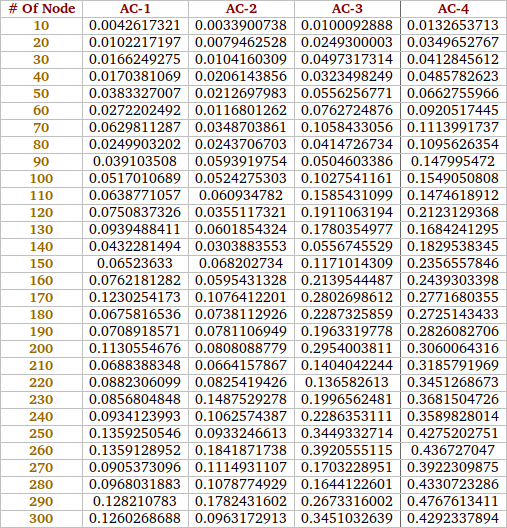
\includegraphics[width=0.48\textwidth]{ac_timeStat}

\caption{\scriptsize Execution time of four AC algorithms for increasing number of node.}
\end{figure}
\\
The above figure shows the execution time of all arc consistency algorithms for increasing number of nodes (10, 20,..,300).\\

Figure 2 shows the comparison of four execution times of four AC algorithms. Here we see, almost linear increase of AC-1, AC-2 and AC-4. But AC-3 doesn't hold that property.

\begin{figure}[h]
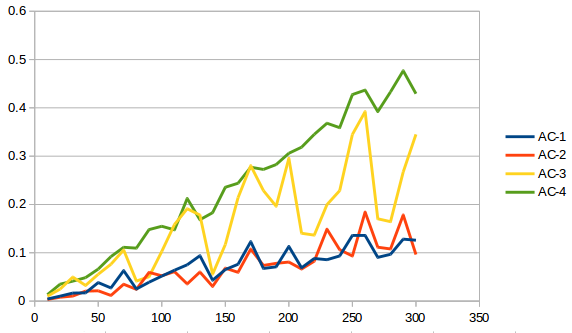
\includegraphics[width=0.48\textwidth]{ac_timeGraph}
\caption{\scriptsize Comparison graph of execution time of ac algorithms for data of Figure 1.}
\end{figure}\\
Figure 3 shows the comparison graph of domain reduction of four AC algorithm v/s number of nodes. AC-1, AC-2 and AC-4 reduces the same number of domain where AC-3 produces result without reducing that large number of domain.\\
\begin{figure}[h]
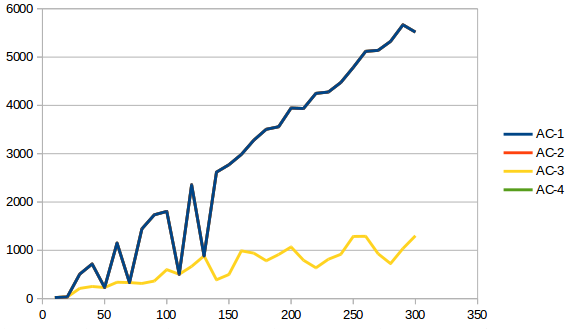
\includegraphics[width=0.48\textwidth]{ac_domGraph}
\caption{\scriptsize Comparison graph of domain reduction of ac algorithms.}
\end{figure}\\\\
\textbf{\large Discussion on Fig-2,Fig-3: }\\
\par From Figure 2, we see that AC-3's graph is changing its slope frequently unlike the other three. This is because AC-3 returns false as long as it finds any domain is zero. But the other three don't return immediately after finding any domain to be zero. Hence, we can guess AC-3 will take less time than the others. But my implementation of AC-3 and AC-4 (iteration through the constraint list) is not so well comparing with the others, thus these two are taking a little longer time comparing with the other two. \\\\Now from Figure 3, we see AC-1, AC-2 and AC-4 are reducing exactly same number of domains, where AC-3 returns true/false immediately after finding any domain is zero. So, AC-3 reduces less number of domain comparing with other three.
\section*{ANOVA Test Result}
\begin{figure}[h]
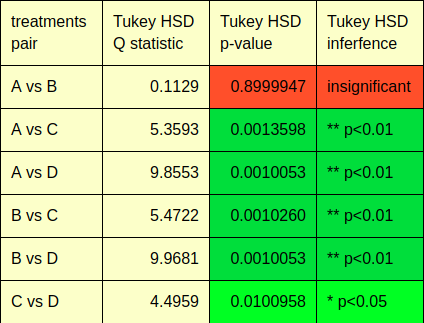
\includegraphics[width=0.48\textwidth]{tukey_HSD}
\caption{\scriptsize Tukey HSD result.}
\end{figure}
Here A,B,C and D respectively denote AC-1, AC-2, AC-3 and AC-4.
\\
\section*{Conclusion}
There is two python file (generateGraph\_028.py and Solution\_028.py). generateGraph\_028.py generates random graph having node number 10, 20, 30,..., 300 and edge number = (node number) $\times$ 1.5, assigns domain and constraint to each variable and arc, following the problem description and write it in Test.txt file. Solution\_028.py reads Test.py and runs all AC algorithms and produces file\_exeTime.txt and file\_domain.txt. file\_exeTime.txt contains all execution time of four algorithm and file\_domain.txt contains number of domain reduction for four algorithms.

\end{document}